\documentclass[crop,tikz]{standalone}
\usepackage{pgfplots}

\usetikzlibrary{arrows.meta}

\pgfplotsset{compat=1.18}

\pgfplotsset{
  inverted/.style = {
    every axis legend/.append style={
      draw=white,
      fill=hardblack,
      text=white
    }
  },
}

\begin{document}
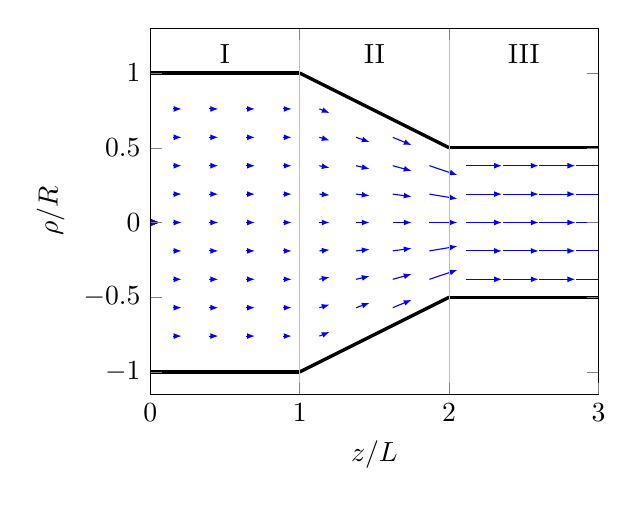
\begin{tikzpicture}
\begin{axis}[
    width={0.6\linewidth},
    view={0}{90},
    axis equal image,
    axis on top=false,
    xmin=0, xmax=3,
    ymin=-1.15, ymax=1.3,
    xlabel={$z/L$},
    ylabel={$\rho/R$},
    xtick={0,1,2,3},
    ytick={-1,-0.5,0,0.5,1},
    xmajorgrids,
    unbounded coords=discard,
    declare function={
        diam(\z)=ifthenelse(\z<1,2,ifthenelse(\z<2,3-\z,1));
        dprime(\z)=ifthenelse(\z<1,0,ifthenelse(\z<2,-1,0));
        radius(\z)=0.5*diam(\z);
        inside(\z,\r)=ifthenelse(abs(\r)<0.92*radius(\z),1,0);
        vz(\z,\r)=inside(\z,\r)*(2/diam(\z))^2;
        vr(\z,\r)=inside(\z,\r)*(4*dprime(\z)/(diam(\z)^3))*\r;
        maskz(\z,\r)=ifthenelse(abs(\r)<0.9*radius(\z),\z,0/0);
        maskr(\z,\r)=ifthenelse(abs(\r)<0.9*radius(\z),\r,0/0);
    },
]
\addplot3[
    blue,
    quiver={
        u={vz(x,y)},
        v={vr(x,y)},
        w={0},
        scale arrows=0.06,
    },
    -{Latex[length=1mm]},
    domain=0.15:2.85,
    y domain=-0.95:0.95,
    samples=12,
    samples y=11,
] ({maskz(x,y)},{maskr(x,y)},{0});
% Wand
\addplot3[black, very thick, domain=0:1, samples=2] ({x},{1},{0});
\addplot3[black, very thick, domain=1:2, samples=2] ({x},{(3-x)/2},{0});
\addplot3[black, very thick, domain=2:3, samples=2] ({x},{0.5},{0});
\addplot3[black, very thick, domain=0:1, samples=2] ({x},{-1},{0});
\addplot3[black, very thick, domain=1:2, samples=2] ({x},{-(3-x)/2},{0});
\addplot3[black, very thick, domain=2:3, samples=2] ({x},{-0.5},{0});
% Abschnittsbeschriftung
\node[above] at (0.5,1) {I};
\node[above] at (1.5,1) {II};
\node[above] at (2.5,1) {III};
\end{axis}
\end{tikzpicture}
\end{document}
